\documentclass[11pt, oneside]{article}   	% use "amsart" instead of "article" for AMSLaTeX format
\usepackage{geometry}                		% See geometry.pdf to learn the layout options. There are lots.
\geometry{letterpaper}                   		% ... or a4paper or a5paper or ... 
%\geometry{landscape}                		% Activate for rotated page geometry
\usepackage[parfill]{parskip}    		% Activate to begin paragraphs with an empty line rather than an indent
\usepackage{graphicx}				% Use pdf, png, jpg, or eps§ with pdflatex; use eps in DVI mode
								% TeX will automatically convert eps --> pdf in pdflatex		
\usepackage{amssymb}
\usepackage{subcaption}


%SetFonts

%SetFonts


\title{Reinforcement Learning Homework 1 : Dynamic Programming and Reinforcement Learning}
\author{Hugo Cisneros}
\date{}							% Activate to display a given date or no date

\begin{document}
\maketitle
\section{Dynamic programming}
\textbf{1.} Optimal policy is [1 1 2], it corresponds to jumping as fast as possible to the state 2 where a reward of 9/10 can reliably be obtained with action 2.
\\

\textbf{2.} $v^* = [15.28615506, 16.44338493, 17.89499783]$
\begin{figure}[h!]
\begin{center}
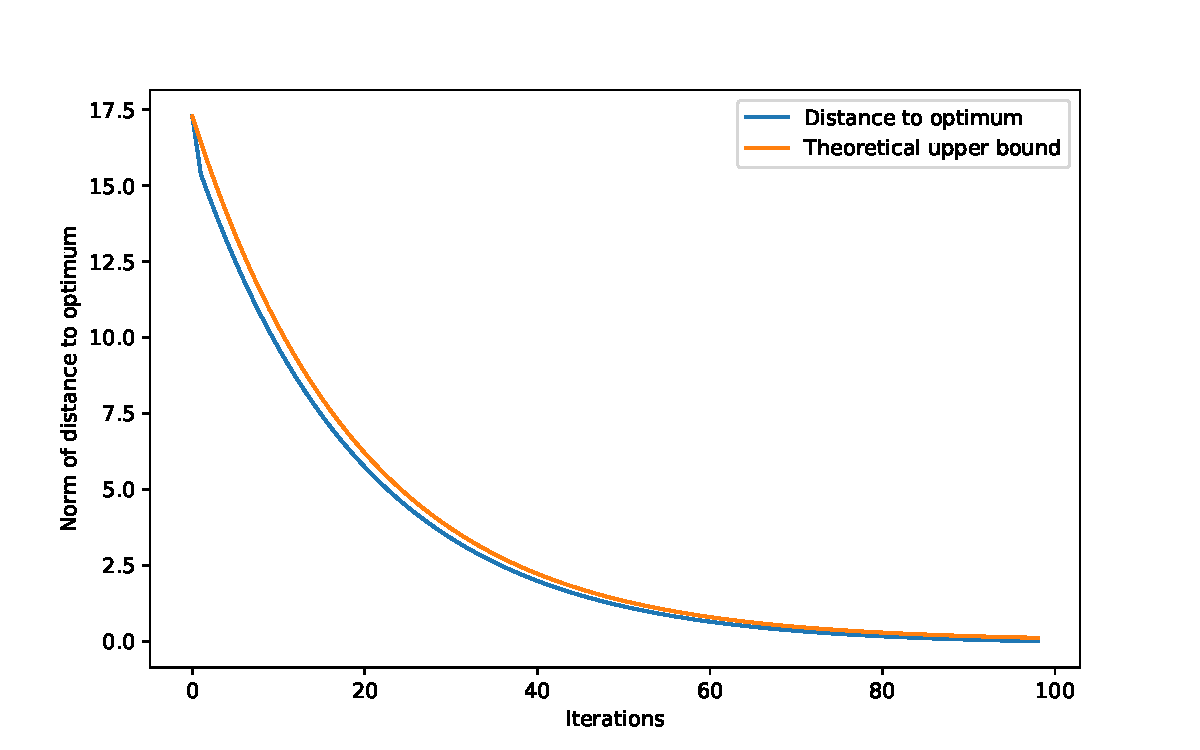
\includegraphics[width=.8\linewidth]{value_iteration.pdf}
\caption{Distance to optimum as a function of number of iterations for value iteration}
\label{default}
\end{center}
\end{figure}

\textbf{3.} Policy iteration converges much faster than value iteration. It only takes 3 steps to reach the optimal policy. However, each of those steps  implies inverting a matrix of size the number of states. This is achieved in $O(n^3)$ time, which isn't significative for such a small problem but becomes prohibitively big for large problems. In that case, value iteration should be preferred. 

%\subsection{}
\section{Reinforcement Learning}
\textbf{1.}
\begin{figure}[h!]
\begin{center}
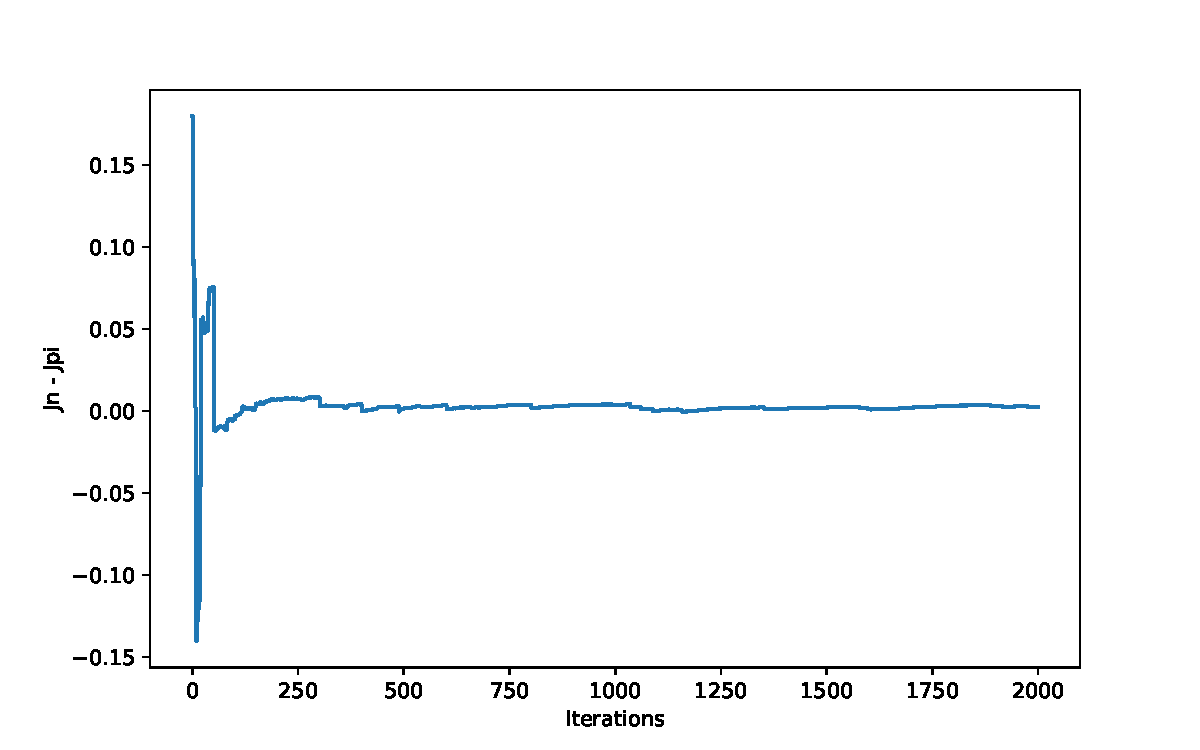
\includegraphics[width=.8\linewidth]{monte_carlo.pdf}
\caption{Gap $J_n - J_{\pi}$ as a function of number of iterations}
\label{default}
\end{center}
\end{figure}

\textbf{2.} The learning rate affects how fast the algorithm converges to a solution (see Figure 3 for illustrations). The closer $\alpha$ is to decaying like the inverse square root, the faster the algorithm converges. The exploration parameters is also very important : for a low $\epsilon$, the algorithm keeps taking the greedy solution and innovates less often, this can be seen on the constant parts of the curve on Figure 3(a). 
Overall, high exploration parameter and learning rate seem to yield the best results for this problem.
\begin{figure}
\centering
\begin{subfigure}{.5\textwidth}
  \centering
  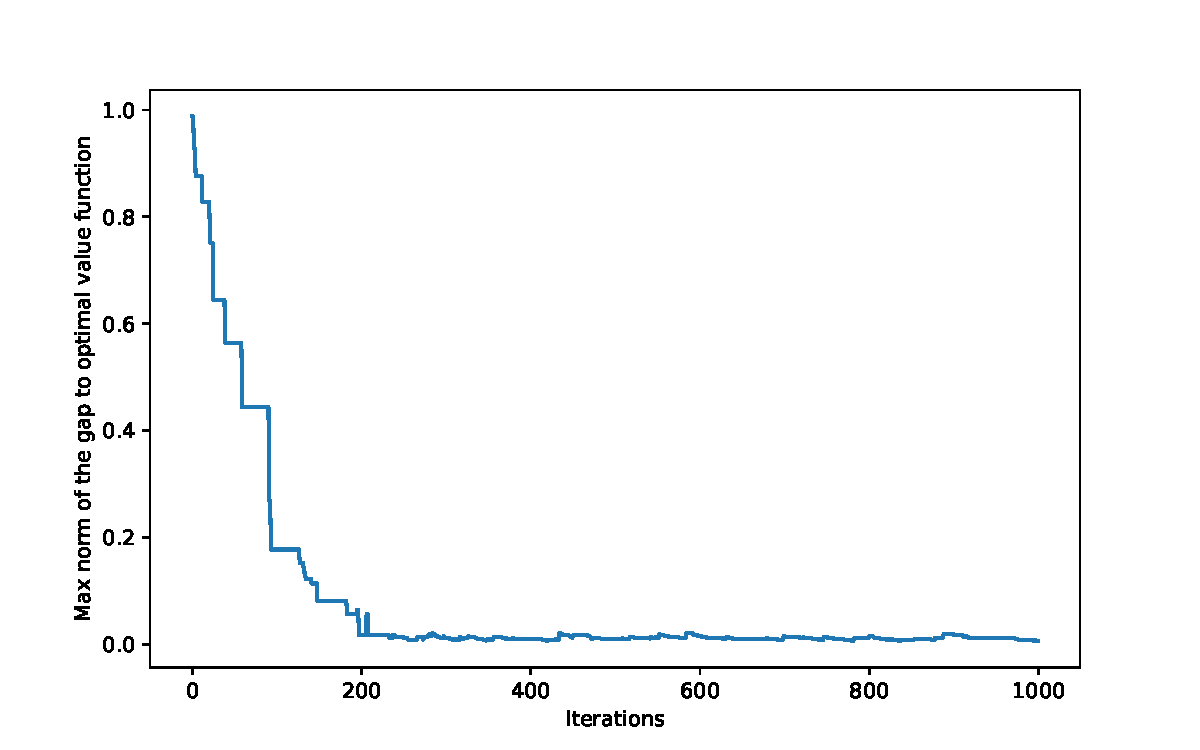
\includegraphics[width=\linewidth]{q_learninge02}
  \caption{$\alpha = \frac{1}{t^{0.51}}, \epsilon = 0.2$}
\end{subfigure}

\begin{subfigure}{.48\textwidth}
  \centering
  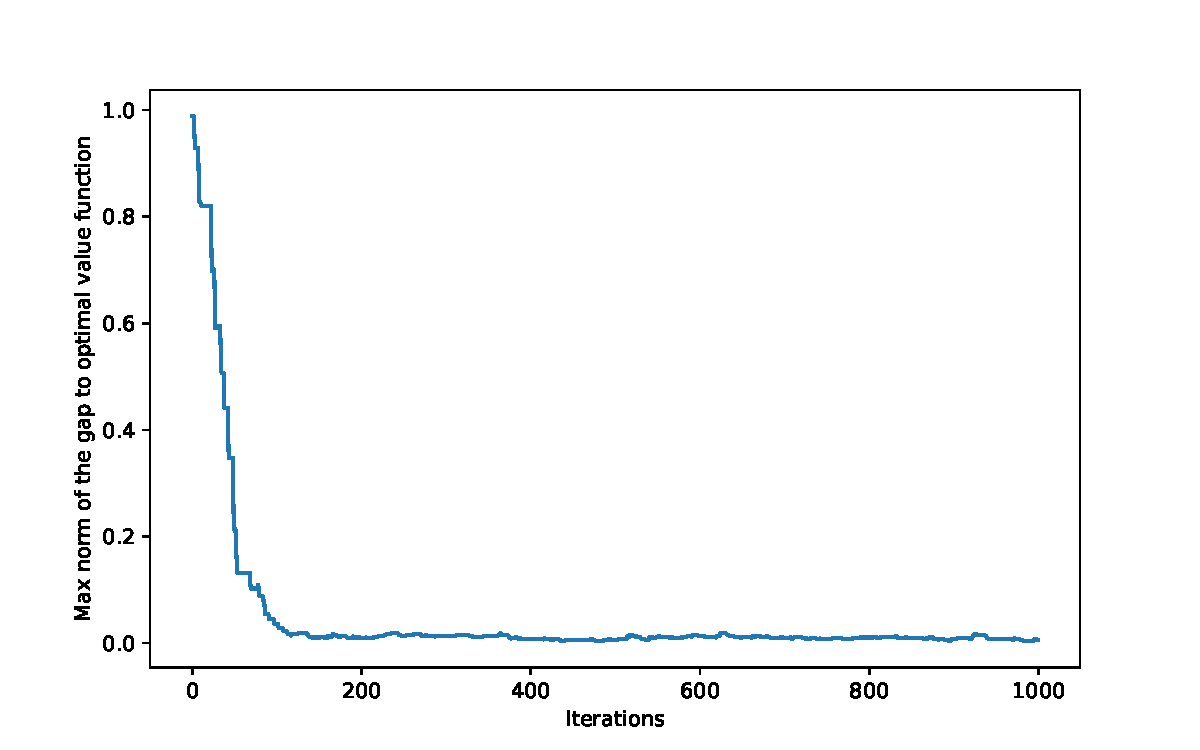
\includegraphics[width=\linewidth]{q_learninge09}
  \caption{$\alpha = \frac{1}{t^{0.51}}, \epsilon = 0.9$}
\end{subfigure}
\begin{subfigure}{.48\textwidth}
  \centering
  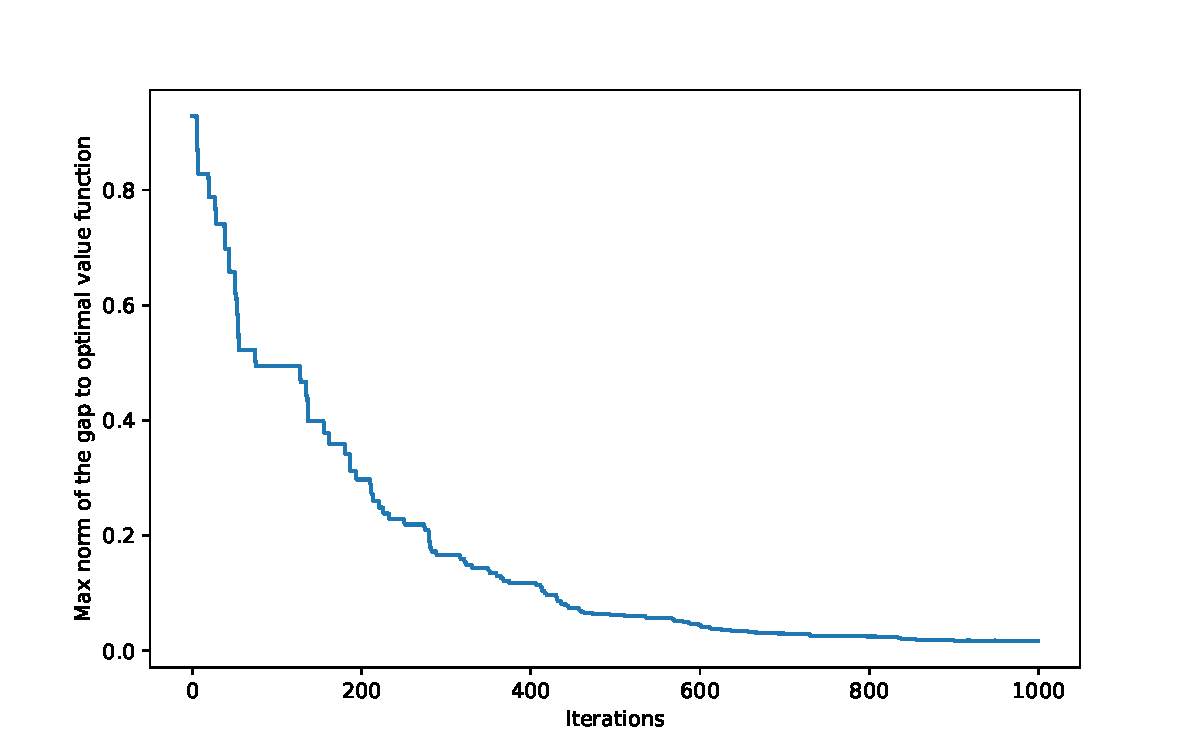
\includegraphics[width=\linewidth]{q_learning08}
  \caption{$\alpha = \frac{1}{t^{0.8}}, \epsilon = 0.5$}
\end{subfigure}
\caption{Comparison of learning rates and exploration parameters for the Q-learning algorithm}

\end{figure}

\begin{figure}[h!]
\begin{center}
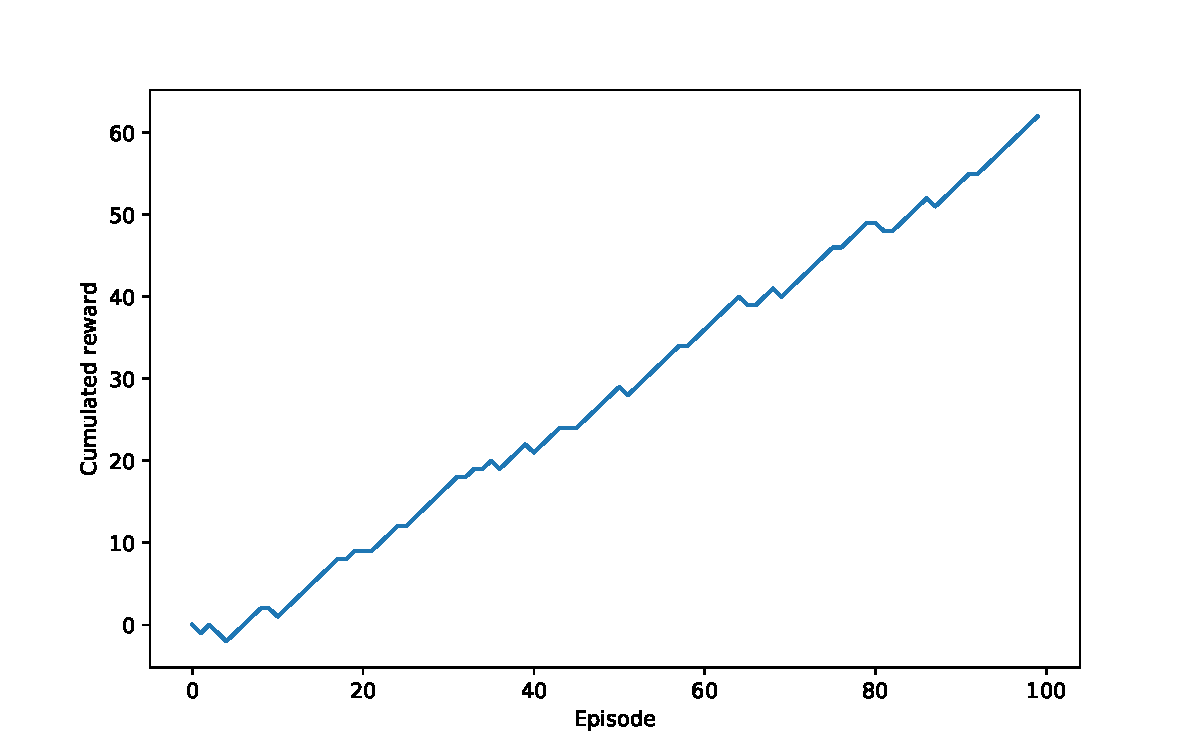
\includegraphics[width=.7\linewidth]{rewards.pdf}
\caption{Evolution of the cumulated reward over the 100 first episodes}
\label{default}
\end{center}
\end{figure}

\begin{figure}[h!]
\begin{center}
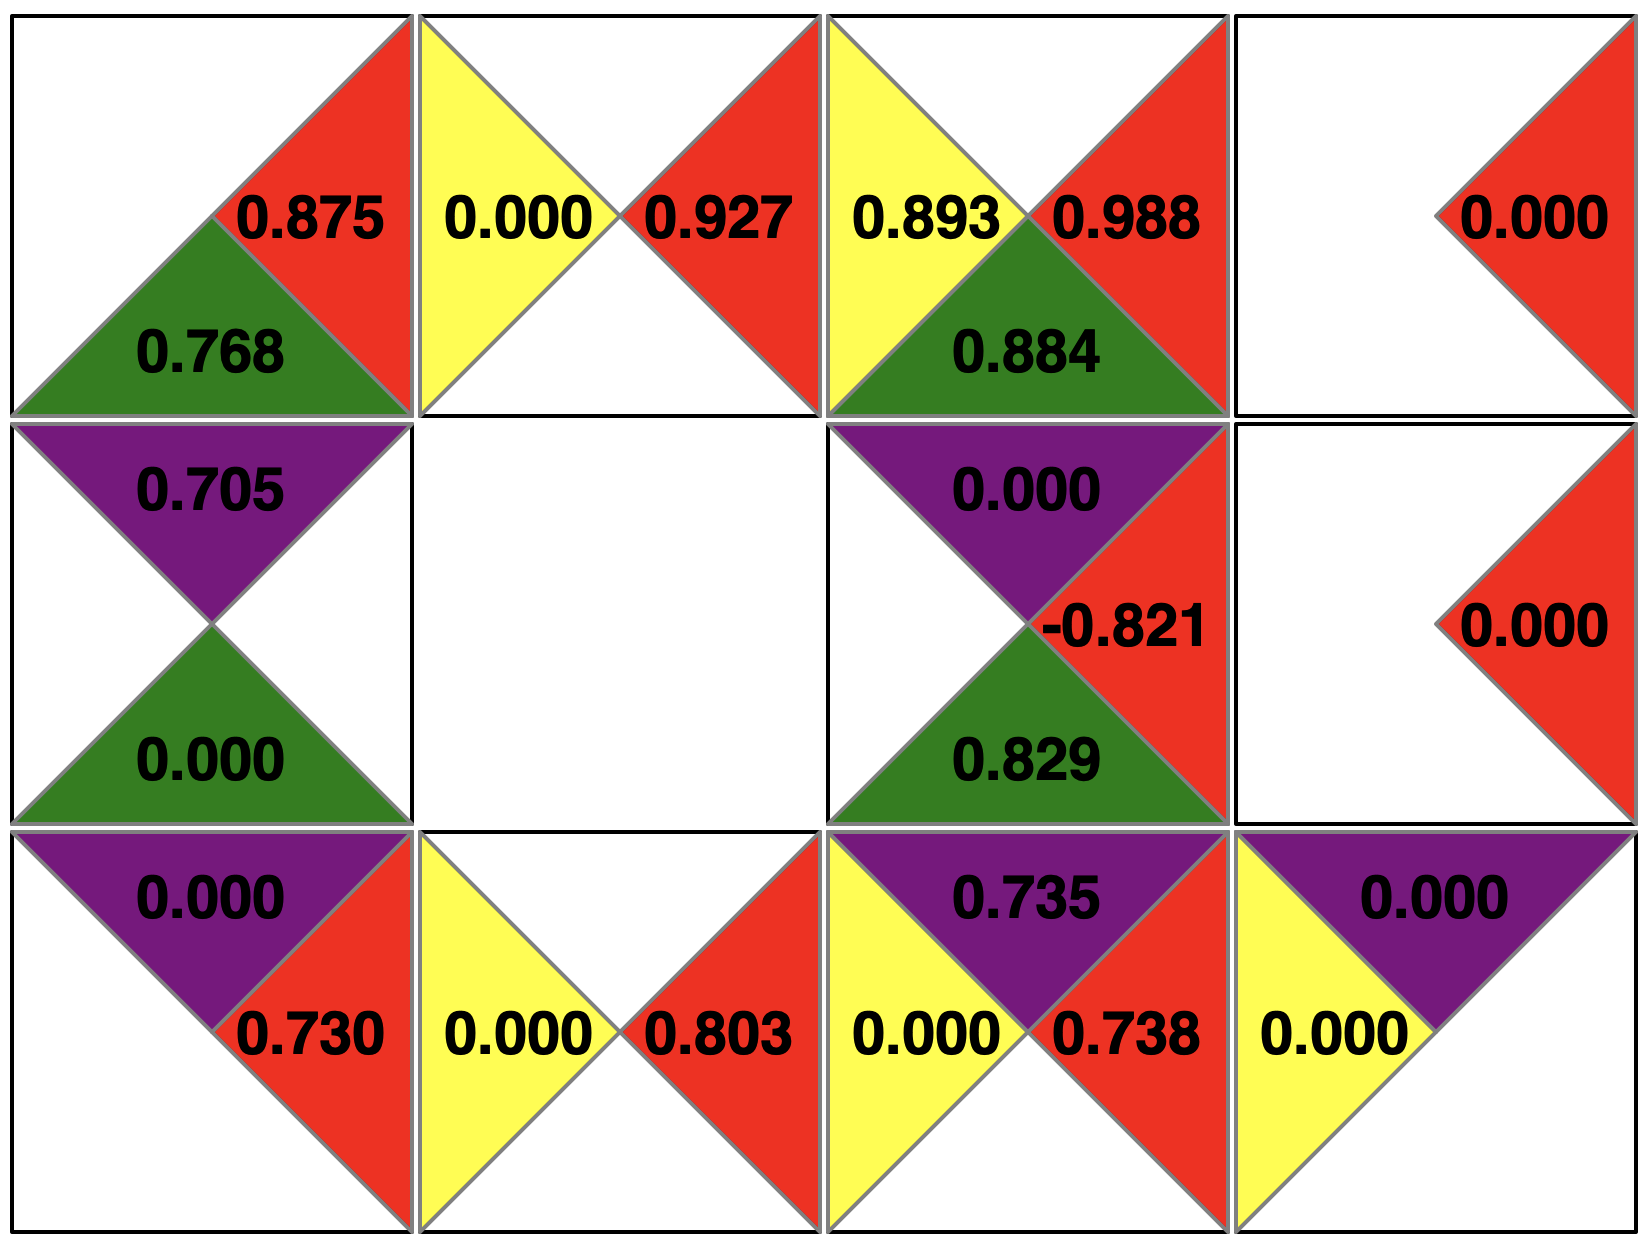
\includegraphics[width=.5\linewidth]{q_final.png}
\caption{Visualization of the final Q function after Q-learning}
\label{default}
\end{center}
\end{figure}



\textbf{3.} The optimal policy doesn't depend on $\mu_0$ since the actions taken depend only on the current state which is not affected by the initial state
\end{document}  